
% \documentclass[a4paper]{article}

% \usepackage{tikz}

% \begin{document}

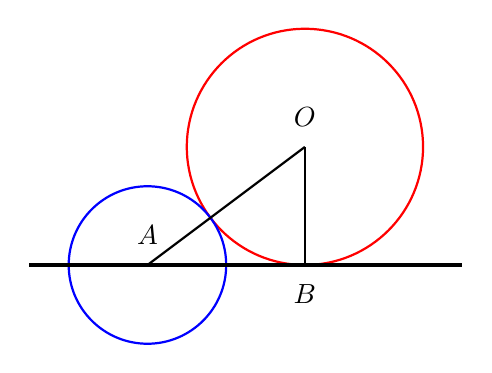
\begin{tikzpicture}[scale = 0.5]
  \draw[red, thick] (4, 3) circle (3cm);
  \draw[blue, thick] (0, 0) circle (2cm);
  \draw[thick] (0, 0) node[label = above: $A$] {}
           --  (4, 3) node[label = above: $O$] {};
  \draw[very thick] (-3, 0) -- (8, 0);
  % \draw (0, 2.25) -- (0, 0) node [label = below: $B$] {};
  \node[label = below: $B$] at (4, 0) {};
  \draw[thick] (4, 0) -- (4, 3);
  % \draw (6, 4   ) -- (6, 0) node [label = below: $D$] {};
\end{tikzpicture}

% \end{document}